\documentclass[12pt]{article}

\usepackage[portuguese]{babel}
\usepackage{float}
\usepackage{array}
\usepackage{listings}
\usepackage{indentfirst}
\usepackage{amsfonts, amssymb, amsmath}
\usepackage{graphicx}
\usepackage{enumitem}
\usepackage[colorlinks=true, allcolors=blue]{hyperref}
\usepackage[letterpaper,
            top=1.5cm,
            bottom=1.5cm,
            left=2.75cm,
            right=2.75cm,
            marginparwidth=1.75cm]{geometry}

\title{Arquitetura e Organização de Computadores I}
\author{Prof. Anderson}
\date{\today}

\begin{document}

\maketitle
\tableofcontents

\vspace{16pt}
OBS.: As primeiras anotações serão da aula do professor Calvo, visto que o 
professor Anderson ainda está em viagem.

\section{Apresentação da Matéria}

\section{Conceitos Básicos}
\begin{itemize}
    \item Arquitetura são os atributos visiveis ao programador
    \begin{itemize}
        \item Conjuntos de instruções, numeros de bits usados para representação 
        de dados, mecanismos de E/S, técnicas de endereçamento.
        \item Exemplo: Existe uma instrução de multiplicação?
    \end{itemize}
    \item Organização é como os recursos são implementados.
    \begin{itemize}
        \item Sinais de controle, interfaces, tecnologia de memória
        \item Exemplo: Existe uma unidade de multiplicação no hardware ou ela 
        é feita pela adição repetitiva
    \end{itemize}
\end{itemize}

Exemplo de Decisão de Projeto
\begin{itemize}
    \item Questão: Presença ou não da instrução de multiplicação.
    \item A decisão deve ser tomada de acordo com: 
    \begin{itemize}
        \item A frequência do uso da instrução
        \item Velocidade relativa das duas técnicas
        \item Custo e tamanho físico de uma unidade de multiplicação especial
    \end{itemize}
\end{itemize}

    \subsection{Função vs Estrutura}
    \begin{itemize}
        \item Função -- É a operação individual de cada componente como parte 
        da estrutura
        \begin{itemize}
            \item As funções do computador são:
            \begin{itemize}
                \item Processamento de dados
                \item Armazenamento de dados
                \item Movimentação de dados
                \item Controle
            \end{itemize}
        \end{itemize}
        \item Estrutura -- É o modo como os componentes são interrelacionados
    \end{itemize}
    \subsection{ENIAC -- Eletronic Numerical Integrator and Calculator}
    \begin{itemize}
        \item Sediado na Universidade da Pensilvânia
        \item É um computador de propósito geral construido entre 1943 e 1946
        \item Realizava cálculos de balística na WW2
        \item Consumiu uma pequena fortuna de \$ 500.000 da época
        \item Ocupava uma área de 150 m$^2$ e pesava 30 toneladas
        \item Era acionado por um motor equibalente a dois potentes motores de 
        carros de quatro cilindros, enquanto um enorme ventilador refrigerava o 
        calor produzido pelas válvulas
        \item Consumia 150.000 watts ao produzir o calor equivalente a 50 
        aquecedores domésticos
        \item Possuia 20 registradores, cada um com capacidade para armazenar 
        um número decimal de 10 algarismos
        \item A programação era feita através de fios e pinos
        \item Executava 5000 adições/subtrações ou 300 multiplicações por segundo
        \item Para programar levava 1 ou 2 dias
        \item Uma grande limitação era a capacidade de armazenamento de dados
    \end{itemize}
    \subsection{John Von Neumann}
    \begin{itemize}
        \item Consultor do projeto ENIAC
        \item Criou o conceito de "programa armazenado"
        \item Criou o conceito de operações com número binários
        \item Desenvolveu a lógica dos circuitos
        \item Memória principal armazenando programas e dados
        \item Unidade de controle interpretando e executando instruções da memória
        \item Criador do modelo de Arquitetura de Von Neumann
        \begin{itemize}
            \item Esta arquitetura foi utilizada no EDSAC, o primeiro computador 
            de programa armazenado
        \end{itemize}
        \begin{figure}[H]
            \centering
            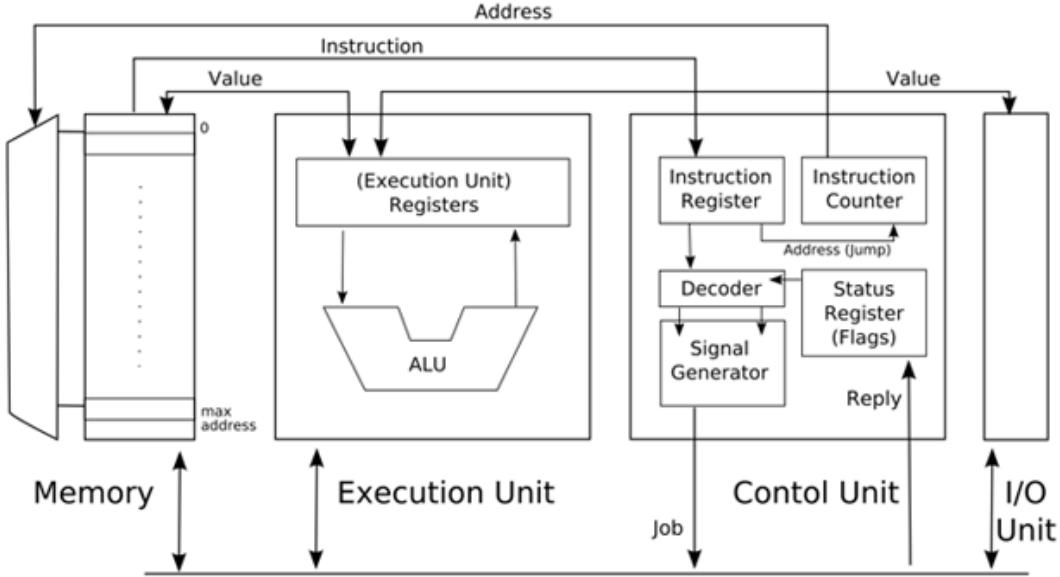
\includegraphics[width=0.65\linewidth]{imagens/arquitetura_von_neumann.png}
        \end{figure}
        \item O modelo de Von Neumann possui cinco componentes principais:
        \begin{itemize}
            \item Unidade de Entrada
            \item Unidade de Saída
            \item Unidade Lógica Aritmética (ULA)
            \item Unidade de Memória
            \item Unidade de Controle (UC)
        \end{itemize}
        \item Memória: 4096 palavras
        \item Cada palavra possuia 40 bits
        \begin{itemize}
            \item Duas instruções de 20 bits
            \item Um dado de 40 bits
        \end{itemize}
        \item ULA + UC = CPU
        \item A Unidade de Controle possuía um registrador de 40 bits (acumulador)
        \item A comunicação entre os componentes é realizada através de um caminho 
        compartilhado chamado barramento de sistema (bus)
        \begin{figure}[H]
            \centering
            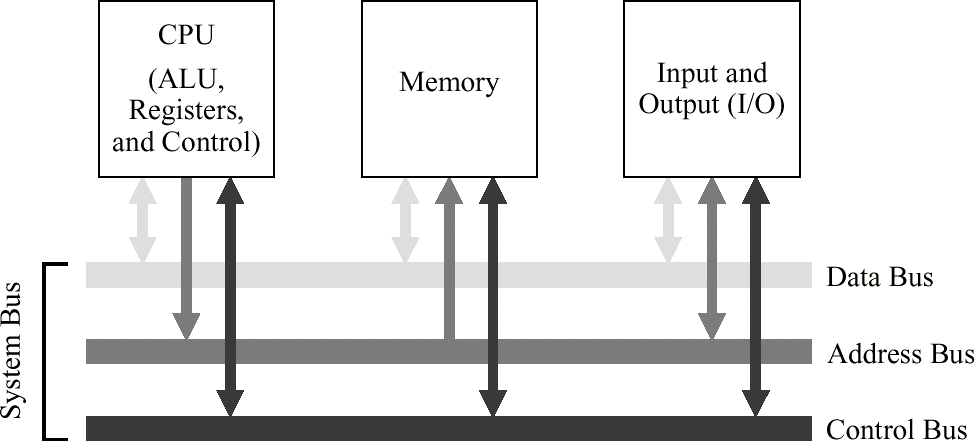
\includegraphics[width=0.75\linewidth]{imagens/bus_arq.png}
        \end{figure}
    \end{itemize}
\section{Estruturas de Interconexão do Computador}
    \subsection{Computador IAS}

    \begin{itemize}
        \item O primeiro computador eletronico, construi
        \item Registradores do IAS
        \begin{table}[H]
            \begin{center}
            \begin{tabular}{|p{6cm}|p{1.75cm}|p{6cm}|}
                \hline
                Registrador & Tamanho (bits) & Função \\ \hline
                
                Contador de Programa (PC) & 12 &  Armazena o endereço da 
                proxima instrução \\ 
                \hline
                Acumulador (AC) & 40 & Armazenamento temporário de dados\\
                \hline
                Multiplier quotient (MQ) & 40 & Armazenamento temporário de 
                dados \\
                \hline
                Buffer de dados/instruções (MBR) & 40 & Dados de 
                leitura/escrita de memória \\
                \hline
                Register de instrução (IR) & 8 & Armazena opcode de uma 
                instrução\\ 
                \hline
                Endereçi de memória (MAR) & 12 & Armazena endereço de 
                memória de uma instrução \\
                \hline
            \end{tabular}
            \end{center}
        \end{table}
        \item Se voce deslocar um numero de bit uma casa pra esquerda, 
        exemplo, 01010 para 10100, é a mesma coisa que multiplicar por 2, 
        se mover para a direita o contrario é verdadeiro.
        \item É possivel colocar um nome para o endereço de memória que começa 
        a função, para que, por exemplo, no jump, seja possivel ir para esse 
        endereço
        \item Arquitetura de Von Neumann
        \begin{itemize}
            \item A Arquitetura de Von Neumann é baseada em 3 conceitos:
            \begin{enumerate}[label=\arabic*)]
                \item Dados e instruções são armazenados em uma mesma memória
                \item O conteudo da memoria é endereçavel sem considerar o 
                tipo de dado
                \item A execução ocorre sequencialmente de uma instrução 
                para outra (exceto que ocorra uma modificação)
            \end{enumerate}
        \end{itemize}
    \end{itemize}
    \subsection{Programação em hardware}
    \begin{itemize}
        \item O armazenamento e operação de dados binários e logicos sao 
        realizados a partir da combinação de componentes logicos
        \item A combinação especifica de componentes logicos pode ser feita 
        para realizar calculos especificos
        \item Conexão de componentes lógicos $\rightarrow$ Programa hardwired
        \item A combinação de componentes logicos pode ser feita para a 
        execução de várias funções (uso geral)
        \begin{itemize}
            \item Sinais de controle são aplicados ao hardware
        \end{itemize}
        \item Ciclo de Instrução
        \begin{itemize}
            \item Um ciclo de instrução é composto por duas etapas
            \begin{itemize}
                \item Ciclo de busca
                \item Ciclo de execução
            \end{itemize}
            \item Ciclo de busca
            \begin{itemize}
                \item Contador de Programa (PC) mantem endereço da proxima 
                instrução a buscar
                \item Processador busca a instrução do local de memoria 
                apontado pelo PC
                \item Incrementar PC -- A menos que seja informado de outra 
                forma
                \item Instrução carregada no Registrador de Instrução (IR)
            \end{itemize}
            \item Ciclo de Execução / instrução
            \begin{itemize}
                \item Processador interpreta instrução e realiza as ações 
                exigidas
                \item Categoria das ações:
                    \begin{itemize}
                        \item Processador -- memória
                        \item Processador -- E/S
                        \item Processamento de dados
                        \item Controle
                    \end{itemize}
            \end{itemize}
        \end{itemize}
        \item Interrupção
        \begin{itemize}
            \item Mecnismo pelo qual módulos (como E/S) podem interromper a 
            sequencia de processamento normal
            \item Interrupções podem ser ocasionadas por:
            \begin{itemize}
                \item Falaha de algum programa: divisão por zero, acesso à 
                espaço de memória inválido, overflow
                \item Timer: sinal para indicar o instante da execução de uma 
                função especifica
                \item E/S: sinalizar o termino de uma operação ou ocorrencia de 
                erros
                \item Falha de hardware: falta de energia
            \end{itemize}
            \item Ciclo de Interrupção
            \begin{itemize}
                \item Adicionado ao ciclo de instrução
                \item Processador verifica Interrupção
                \begin{itemize}
                    \item Indicado por um sinal de Interrupção
                \end{itemize}
                \item Se não houver interrupção, busca próxima instrução
                \item Se houver interrupção pendente:
                \begin{itemize}
                    \item Suspende execução do programa atual
                    \item Salva contexto
                    \item Define PC para endereço inicial da rotina de 
                    tratamento de interrupção
                    \item Interrupção do processo
                    \item Restaura contexto e continua programa interrompido
                \end{itemize}
            \end{itemize}
            \item Multiplas interrupções
            \begin{itemize}
                \item Desativar Interrupções
                \begin{itemize}
                    \item Processador ignorara outras interrupções enquanto 
                    processa uma interrupção
                    \item Interrupções permanecem pendentes e são verificadas 
                    após a primeira interrupção ter sido processada
                    \item Interrupções tratadas em sequencia enquanto ocorrem
                \end{itemize}
                \item Definir prioridades
                \begin{itemize}
                    \item Interrupções de baixa prioridade podem ser 
                    interrompidas por interrupções de prioridade mais alta
                    \item Quando a interrupção de maior prioridade tiver sido 
                    processada, processador retorna à interrupção anterior
                \end{itemize}
            \end{itemize}
        \end{itemize}
    \end{itemize}
\end{document}